% Titelgrafik der Programmier-Folien: sieben Emoji-Spiralen wie \makeSpiral
% (Preambles/pre_5_misc.tex), hier als normales Bild in Textbreite statt als Overlay.
% Ersetzt die frühere Rastergrafik title-emojis.jpg (Apple-Emojis, nicht frei lizenziert);
% \emoji{} verwendet Noto Color Emoji (Google, Apache License 2.0).
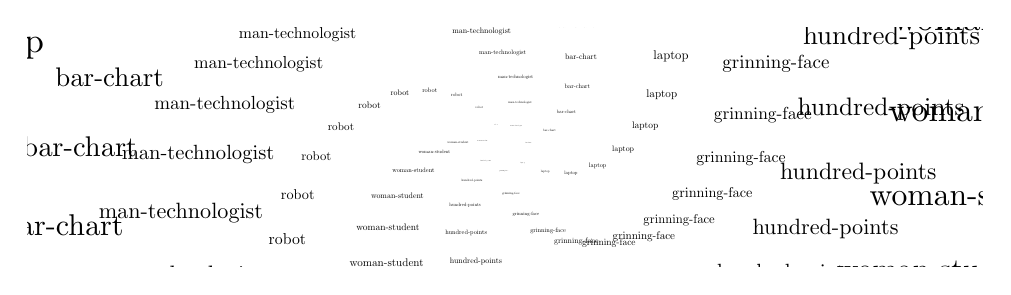
\begin{tikzpicture}
	% sichtbarer Ausschnitt: volle Textbreite, ein Viertel davon hoch
	\clip (-.5\textwidth, -.125\textwidth) rectangle (.5\textwidth, .125\textwidth);
	\foreach \theemoji [count=\nSpiral] in {man-technologist, robot, woman-student, hundred-points, grinning-face, laptop, bar-chart} {
			% jede Spirale beginnt um 360/7 Grad versetzt
			\pgfmathsetmacro{\startAngle}{\nSpiral/7*360}
			% gleiche Werte wie \makeSpiral; ab \i = 22 liegen alle Emojis ausserhalb des Ausschnitts
			\foreach \i in {1,...,22} {
					% Winkel, Abstand und Grösse wachsen mit \i: kleine Emojis innen, grosse aussen
					\pgfmathsetmacro{\angle}{\startAngle + \i*10}
					\pgfmathsetmacro{\radius}{0.3*\i}
					\pgfmathsetmacro{\scale}{4*\i/70}
					\node[scale=\scale, inner sep=0pt] at (\angle:\radius) {\emoji{\theemoji}};
				}
		}
\end{tikzpicture}
